\chapter{Model Inspection}
\label{ch:model-inspection}

Here's another interesting combination of widgets: \widget{Tree Viewer} and \widget{Scatter Plot}. In Scatter Plot, find the best visualization of this data set, that is, the one that best separates instances from different classes. Then connect Tree Viewer to Scatter Plot. Selecting any node of the tree will output the corresponding data subset, which will be shown in the scatter plot.

\begin{figure}[h]
    \centering
    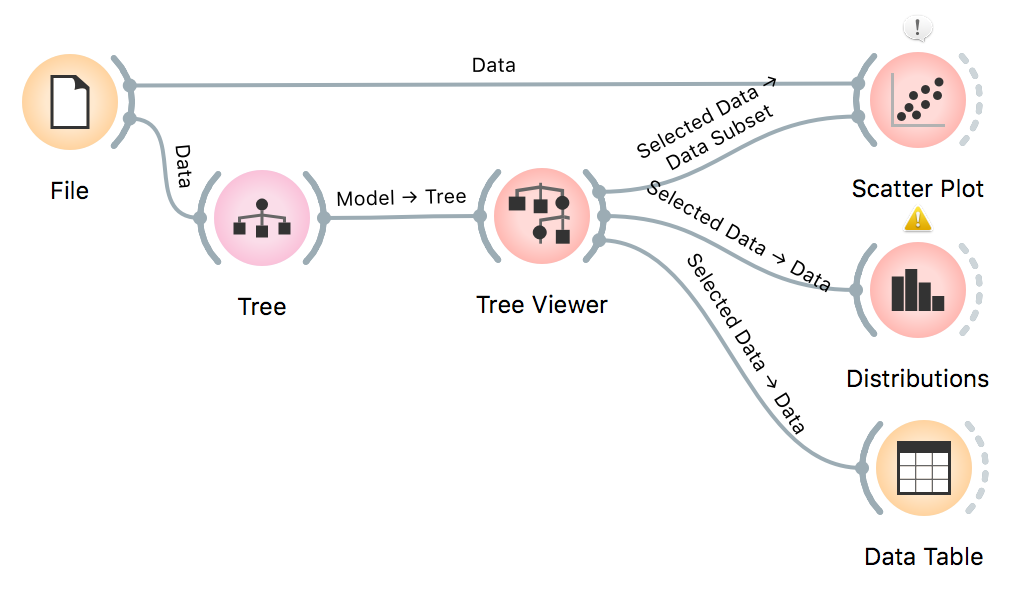
\includegraphics[width=\linewidth]{workflow.png}
    \caption{$\;$}
\end{figure}

\begin{wrapfigure}{o}{1.0\textwidth}
    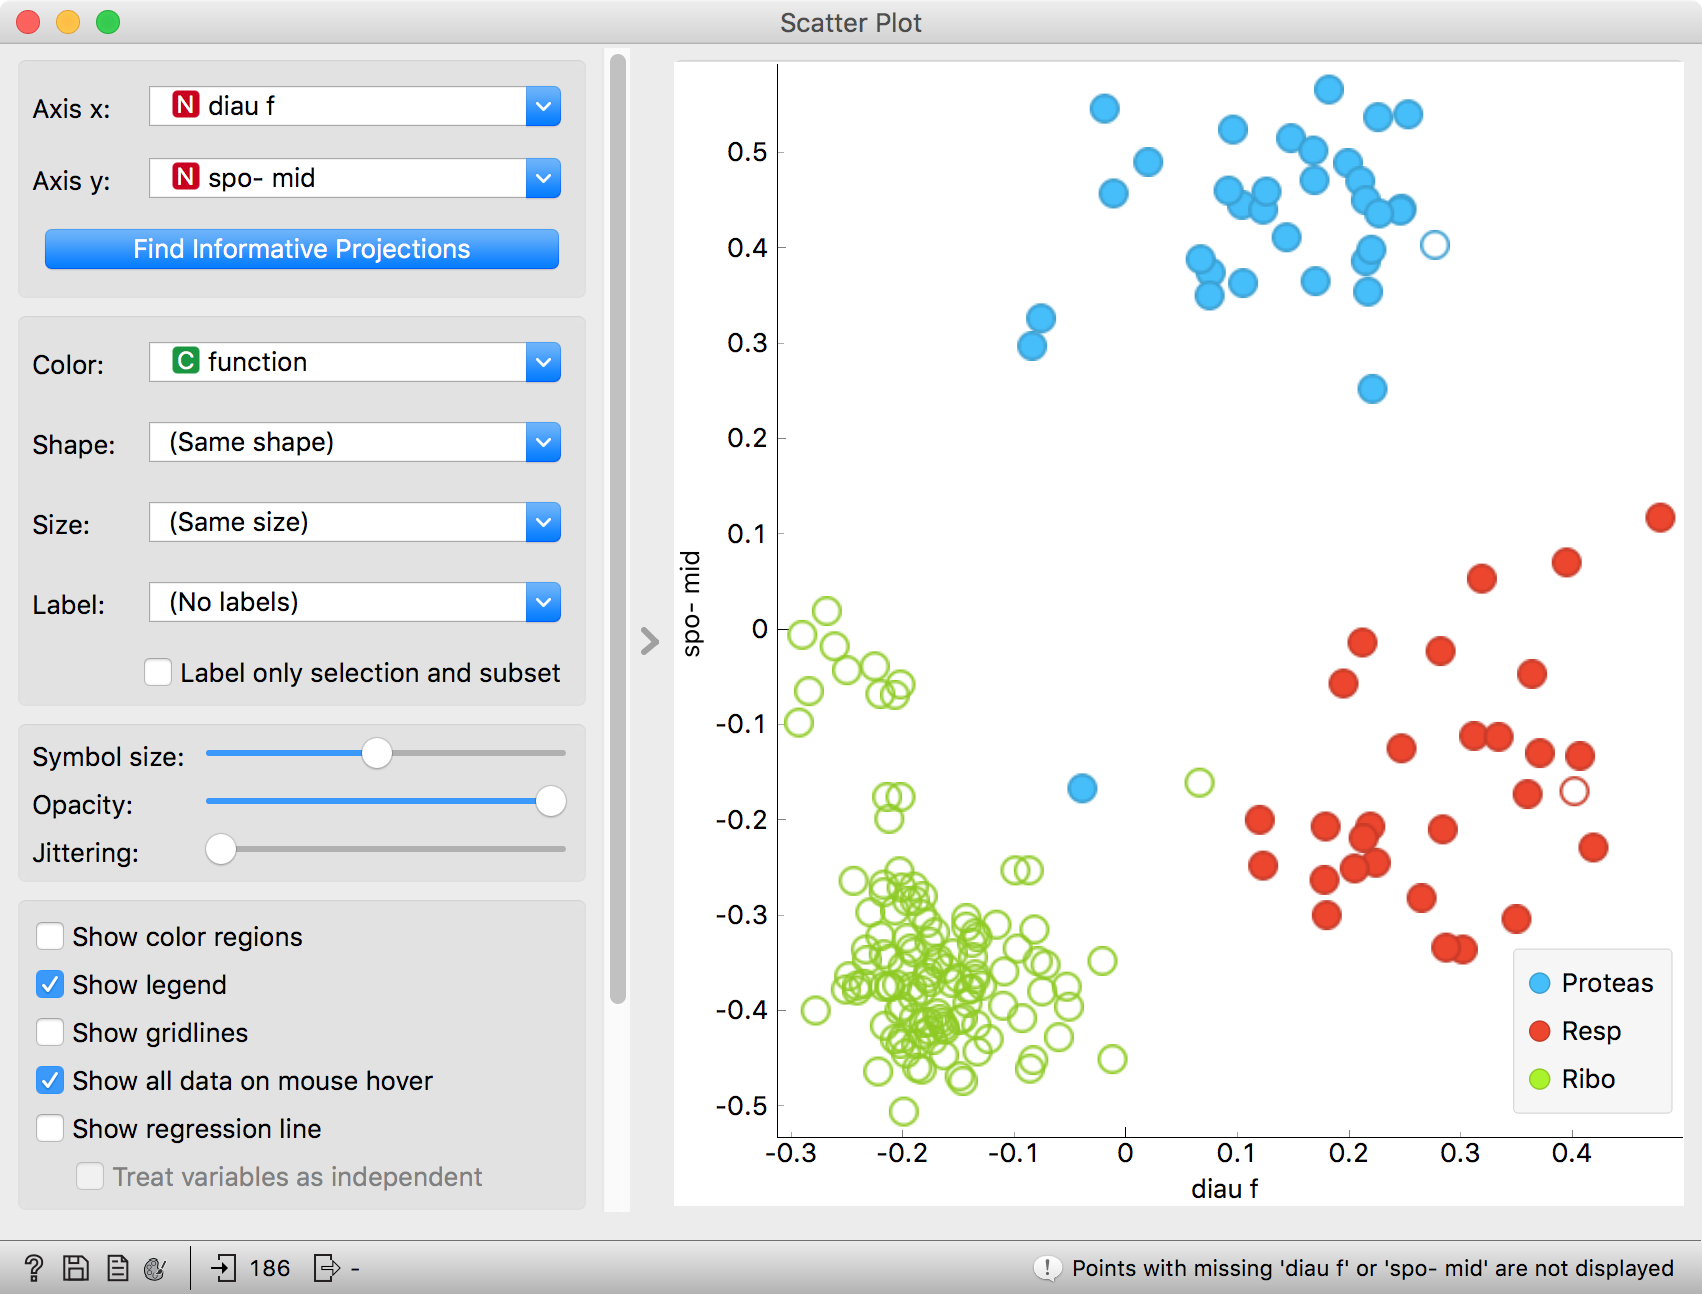
\includegraphics[scale=0.35]{brown-scatterplot.png}
    \label{fig:scatterplot}
\end{wrapfigure}

Just for fun, we have included a few other widgets in this workflow. The Tree Viewer selects data instances by inferring rules from the data itself and optimizing to obtain purer data subsets.
